% Copyright (C) 1988, 2010 Oren Patashnik.
% Unlimited copying and redistribution of this file are permitted if it
% is unmodified.  Modifications (and their redistribution) are also
% permitted, as long as the resulting file is renamed.
\documentclass[11pt]{article}
\usepackage[left=2.5cm, right=2.5cm, top=2cm]{geometry}
\usepackage{multicol}
\usepackage{caption}
\usepackage{graphicx}
\usepackage{amsmath}
\usepackage{lineno, blindtext}

\def\BibTeX{{\rm B\kern-.05em{\sc i\kern-.025em b}\kern-.08em
    T\kern-.1667em\lower.7ex\hbox{E}\kern-.125emX}}

\title{A Novel Technique of Vision-Based Pineapple Crown and Fruit Recognition for Ripeness Index Classification}
\author{Mochammad Fatchur Rahman \and
	 	Kudang Boro Seminar \and 
	 	Mohamad Solahudin \and
 		Supriyanto}

\date{}
\providecommand{\keywords}[1]{\textbf{\textit{Keyword---}} #1}

\begin{document}
\begin{linenumbers}
\maketitle
\begin{abstract}
	Generally, research of vision-based pineapple grading is by cutting the crown first. It makes the pineapple rot quickly. For this reason, this paper presents a breakthrough that makes the computer able to distinguish the crown and fruit automatically. Hence the farmer doesn't need to cut the crown for their vision-based classification machines. This capability also facilitates further feature extractions for ripeness classifications. The first step is the pineapple image acquisition. The next is searching the dividing line between the crown and fruit from the image. It divides the pineapple into two and passes a curve between the crown and fruit, also crosses the pineapple orientation perpendicular.
	Moreover, The pineapple orientation took from PCA analysis. After the pineapple separated into two parts, each part is analyzed morphologically. In this study, compactness is a selected morphological feature. The region with higher compactness considered as the fruit region, and other as the crown. The recognition accuracy of this technique is 98.92\texttt{\%} with 98.92\texttt{\%} of recall. Thus, this technique considered as an excellent approach to recognize the fruit and crown region of a pineapple. After that, this study extracts the color feature for the classification input and artificial neural networks as the classifier. The ripeness standard of this paper refers to the Sunpride standard, the third-largest pineapple producer in the world. This system can classify the pineapple ripeness level with 93.33\texttt{\%}  of test accuracy. The restriction of this study is the background color should be homogeneous.
\end{abstract}

\keywords{Vision Based, Pineapple Detection, Ripeness index classification}

\section{Introduction}

Agriculture is the main livelihood of the population of developing countries, including Indonesia. Their primary agricultural commodities are fruits, vegetables, and crops. In fruits commodities, pineapple is a pre-eminent commodity in Indonesia. Ministry of Commerce of the Republic of Indonesia recorded the export of pineapple in 2013 was 0.897 billion, the second-largest exporter in the world with a market share of 28.43\texttt {\%} \cite{pineapple-export-kemendag}. Besides, the Central Statistics Agency of the Republic of Indonesia noted that pineapple productivity in 2017 reached 1,795,985 tons \cite{BPS-website}. This commodity is the highest production compared to other horticultural products. Pineapple must have certain quality To pass the export standards in terms of size, maturity, and appearance. Therefore a consistent, low-cost, and computer-based grading system is required for subsistence farmers or home industries.

Researchers have done a lot of study on computer-based pineapple post-harvest handling. Moonrita et al. \cite{pineapple-detection-moonrita} developed an on-farm or outdoor pineapple detection method. This study was limited to pineapple detection without separating the fruit and crown. Their features were SIFT, SURF, and Harris with the same descriptor. The detection capability of this research is 82\texttt {\%}, without specifying the value of test or training accuracy. This result is certainly less than ideal for on-farm application. Kaewapichai \cite{pineapple-grading-kaewapichai} researched to reconstruct patterns on the surface of a pineapple. This study needs to cut the crown first, also preliminary research of the pineapple grading. The low-quality pineapple has a lousy pattern due to many wrinkles, and vice versa. In describing the pineapple pattern, They used a snake or active contour algorithm. The achievement of this research is only the image processing to process the pineapple pattern without producing quantitative data. So it has not yet provided a quality conclusion. 

Mohammad S \cite{Mohammad:2011} from Pahang Malaysia developed an image-based pineapple-grading system using the yellowish presentation. The weakness of their research is the crown cutting first and make pineapple rot quickly due to bacterial infections. The study used manual thresholds to determine quality. The same work was done by Ansor JI \cite{anshor:2013} using red (R), green (G), blue (B) features and neural network as a classifier. Similar to Mohammad S research, Ansor JI requires the pineapple crown cutting first. As a result, the fruit is rot quickly. Phataveerat S \cite{Phataveerat:2008} classified the quality of pineapple using sound waves. Although this method does not need to cut the crown first, but not applicable, the reason is the room should be conditioned as quiet as possible, so the outside noise does not affect the result of classification.

Other than pineapple, nondestructive evaluation method has been developed for other commodities, such as a tomato classification using optical absorption features \cite{Zhu:2015}, date fruit hardness with edge detection algorithms \cite{Manickavasagan:2013}, and apple classification using Otsu method and support vector machine \cite{Mizushima:2013}. Furthermore, Rivera NV \cite{Rivera:2014} used K-NN to analyze the physical damage of mangoes, while Payne A \cite{Payne:2014} developed an outdoor mango segmentation technique using Hessian filters to predict the crop yield. Cubero S \cite{Cubero:2014} utilized the standard citrus index features for indoor orange quality evaluations. Then, Sengupta S \cite{Sengupta:2014} developed a technique for the same outdoors work with SIFT features and SVM classifiers. Lastly, Font D \cite{Font:2014} used artificial lights and grayscale normalization methods for grapes harvest valuations at night.

\begin{tabular}{ p{0.2cm} p{1.7cm} p{1.5cm} p{1.8cm} p{2.8cm} p{2.5cm} p{1.6cm} p{0.5cm}}
	\hline
	No & Author & Commodity & Features & ML Algorithms & Scoope & indoor /outdoor & FPS\\
	\hline
	1. & Moonrita (2010)    & Pineapple & SIFT, SURF         & SIFT, SURF       & Detection               & Outdoor & -\\ 
	2. & Kaewapichai (2006) & Pineapple & Color              & Manual threshold & Grading                 & Indoor  & 3\\
	3. & Kaewapichai (2007) & Pineapple & Skin pattern       & Snake            & Just an image processing& Indoor  & -\\
	4. & Mohammad S (2011)  & Pineapple & Color              & Manual threshold & Grading                 & Indoor  & -\\
	5. & Ansor JI (2013)    & Pineapple & Color              & Neural network   & Grading                 & Indoor  & -\\
	6. & Proposed           & Pineapple & Compactness and color & Neural Network& Detection and grading   & Indoor  & 18-33\\
	\hline
\end{tabular}

Based on \textbf {Table 1},vision-based pineapple classification research requires the crown cutting first. Therefore, making the computer capable of recognizing the crown and the fruit region by itself is the novelty offered in this study. Such capabilities are not limited to specific orientations. So the pineapple image acquisition by the camera does not need to be set in such a way that the position of the pineapple in the image looks vertical or horizontal.

This study adopts morphological feature to recognize the crown and the fruit of a pineapple. Morphological features provide necessary object information. This feature can be a proportion of length to width, a ratio of length to the area, center of gravity, roundabout, shrinkage, eccentricity, smoothness, symmetry, elongation, ferret coefficient, and fractal value. Some studies used these features to recognize an object, such us classify weeds and main crops, identify fruit types, and grain varieties. Astrand B \cite{Astrand:2002} applied roundness and elongation features for the identification of main crops and weeds in agricultural robots. Zapotoczny P \cite{Zapotoczny:2008} used a combination of morphological features for the classification of grain varieties. Cubero S \cite{Cubero:2014} used compactness features for grape quality analysis. Boniecky P \cite{Boniecki:2015} applied a form feature for insect identification. Boniecky P describes the shape ratio (compactness) as the ratio of perimeter to the area of the object area \cite{Boniecki:2015}.
\begin{equation}
	R_s=\frac{L^2}{4\mu s}
\end{equation}
However Nixon MS (2002) \cite{Nixon:2013} describes the compactness as a ratio between the area with the squared perimeter.
\begin{equation}
	R_s=\frac{4 \mu A}{P^2}
\end{equation}
Same definition is also used by Persson M (2008) \cite{Persson:2008}, and Arribas JI (2011) \cite{Arribas:2011}. 

\section{Materials And Methods}
In this section, this paper will present the end to end vision-based pineapple quality evaluation from image acquisition to ripeness classification. So there are three main subtopics, that are image acquisition, pineapple crown and fruit separation, and ripeness classification.

\subsection{Image Acquisition }
This research requires a homogeneous and white background for image acquisition. The camera is a 640 x 480 pixel CMOS camera with an illumination lamp of 550 - 600 lux. For real-time image processing, this study used a computer with 2.8 GHz of CPU and 8 GB of RAM. Especially for background color, not necessarily white. The background color can be with other colors but homogeneous, bright and distinctive with pineapple colors. An explanation of this reason is in the next section. The homogenous color here means the background does not have to be uniform. A homogeneous environment with small spots or soft gradations is acceptable because before being processed, this study transformed the image into blurry. Gradations or low spots on the background will disappear. The background color is the limitation of this study.  We also set the light from any direction during image acquisition to minimize the shadow effect. Our method designed for orientation invariant, so there is no restriction for pineapple orientations.

\subsection{Pineapple Crown and Fruit Recognition}
This section will focus on explaining image processing methods to separate the crown and the fruit region of pineapple. There are some steps for this subtopic, shown by {Figure 1}. 
\begin{center}
	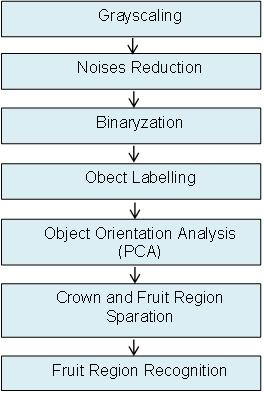
\includegraphics[scale=0.73]{images/flowchart}
	\captionof{figure}{Fruit Detection Flowchart}
\end{center}

\subsubsection{Grayscaling}
The camera captured an image, then stored it as a matrix A. This matrix consists of three channels, namely red, green, and blue channels. The next step is converting this image into a grayscale image. The general formula of grayscale conversion is as follows.
\begin{equation}
	B_ij=\frac{r + g + b}{3}
\end{equation}
where r, g, and b are the values of the blue, green and red channels in Matrix A, while B is the resulting grayscale image.

\subsubsection{Noises Reduction}
This research performed an image noise reduction using a moving average or box filter. The box filter works by averaging the pixel values in (kxk) sub-window (Szelisky, 2011) \cite{Szeliski:2011}. The following convolution operation is the equation of the resulting image.

\begin{equation}
	B = F(x) * B
\end{equation}
Where \(F(x)\) is the box filter applied.

\subsubsection{Binarization}
This research converted the grayscale image (matrix \(B \)) into a binary image using the Otsu method. This method works by compiling the image histogram. Then, we utilized the histogram for separating the image into two groups based on the local minimum between two histogram peaks. The first group is the object representation, then changed to white. The second is the background representation and changed to black or vice versa. The reason for the background color should be homogeneous and bright is to have clear histogram pattern, so the resulting binary image will be better. If the background color is not uniform, there will be many peaks scattered on the image histogram, and generate poor binary images. It is also possible to use a dark background color. However, the color must be very thick, and the object must be brighter for achieving an excellent binary image. Poor binary images will produce imperfect classifications. This paper denotes binary images as matrix \(B \).

\subsubsection{Object Labelling}
Our study utilized a flood fill algorithm for the object labeling of the binary image. This method recognizes the white pixels (255) and interconnected each other as a single object. After that, the pixel positions of the object were extracted. From this process, we got two vectors. The first vector contains the object pixel positions corresponding to the x-axis and the second for the y-axis. In this paper, both vectors are symbolized as vectors \textbf{a} and \textbf{b}. The purpose of this process is for getting the Region of Interest (ROI) for each object.

The region of interest (ROI)  is a square area whose two corners are at the tip of the object. If two edges of the object are symbolized as points \(P1 \) and \(P2 \), then \(P1 \) and \(P2 \) can be formulated as follows,
\begin{multicols}{2}
	\begin{equation}
		\begin{split}
			P1.x &= min(\textbf{a}) \\
			P1.y &= min(\textbf{b}) \\
		\end{split}
	\end{equation}
	\begin{equation}
		\begin{split}
				P2.x &= max(\textbf{a}) \\
				P2.y &= max(\textbf{b}) 
		\end{split}
	\end{equation}
\end{multicols}

\begin{center}
	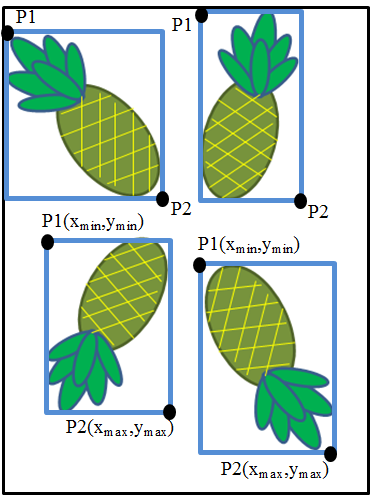
\includegraphics[scale=0.65]{images/object-roi}
	\captionof{figure}{Illustration of ROI}
\end{center}		
Figure 2 shows the ROI of each object. Once the object ROIs were known, the color image from matrix \(A\) was cropped on each ROI. The results of this process are some small images. Then we symbolize them as matrix \(C^{(i)}\) as much as n units. \(C^1\) represents the matrix of the first object ROI, while \(C^n\) is the matrix of the n-th object ROI. Then, the matrix \(C\) is grouped in a vector. This paper symbolizes it as \(\textbf{c}\).

The similar approach is conducted for the binary image or the matrix \(B\), The results of this process are also some small images. This paper symbolizes it as the \(D^{(i)}\). \(D^ 1\) represents the matrix of the first ROI from the binary object, while \(D^n\) represents the matrix of the n-th binary object ROI. Then, the \(D\) is grouped in the vector \(\textbf{d}\).

\begin{multicols}{2}
	\begin{equation}
		\begin{split}
			\textbf{c} = \begin{bmatrix}
				C^1 \\
				C^2 \\
				\vdots \\
				C^n
			\end{bmatrix}
		\end{split}
	\end{equation}
	\begin{equation}
		\begin{split}
			\textbf{d} = \begin{bmatrix}
				D^1 \\
				D^2 \\
				\vdots \\
				D^n
			\end{bmatrix}
		\end{split}
	\end{equation}
\end{multicols}


\subsubsection{Object Orientation Analysis}
Each ROI of the binary object from the previous section or vector \(\textbf{d}\) was conducted further analysis to get object orientation. The orientation analysis was done using principal components analysis (PCA). In this case, the object orientation is the eigenvector with the largest eigenvalue, while the object midpoint is the mean of the PCA.
\begin{center}
	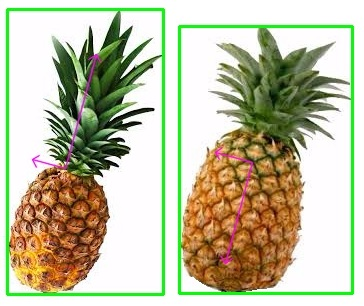
\includegraphics[scale=0.73]{images/pca}
	\captionof{figure}{The Main Componens from PCA of Pineapple Pixels (Red Arrow)}
\end{center} 
The illustration above shows that the X’-axis is the primary orientation of the object or eigenvector with the largest eigenvalue. Y’-axis is the axis perpendicular to the X’-axis, and O’ is the object center point or mean. By knowing the object orientation, we found a new coordinate system with X’ and Y’ axes centered on O’. This new coordinate system facilitates the searching of the curve between the fruit and the crown. This curve is used as a separator of both regions.

\subsubsection{Crown and Fruit Region Sparation}
The dividing line divides the fruit and crown at the curve between both. Therefore, this line is perpendicular to the orientation of the object or X'-axis. Thus, the separation of the fruit and crown will be easier by using this new coordinate system. A coordinate system with X' and Y'-axes, and the center point O' as described in the previous discussion.
\begin{center}
	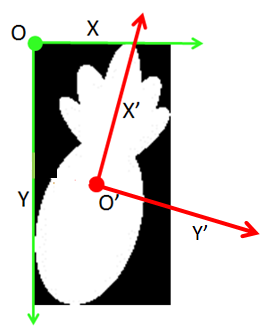
\includegraphics[scale=0.4]{images/two-coordinate-systems}
	\captionof{figure}{Illustration of initial coordinates system with green color and new coordinates system with red color}
\end{center}
 A geometric transformation was applied to get the position of the object pixels based on the new coordinate system. But in this case, the transformation is not on the object, but the coordinate system is. Therefore, it needs a little modification of standard transformation equations. The first process is the shift of the initial coordinate axis (green color) from point O to O', so the operation is a translation.
\begin{center}
	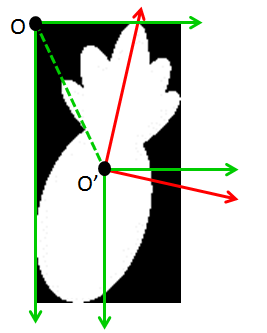
\includegraphics[scale=0.4]{images/translation}
	\captionof{figure}{Coordinates Translation}
\end{center}
Taking point O as point (0,0) and O' as point (a, b), the object pixel positions are formulated as follows,
\begin{equation}
	\begin{bmatrix}
		x_{new} \\
		y_{new}
	\end{bmatrix} = \begin{bmatrix}
	x - a \\
	y - b 
\end{bmatrix}
\end{equation}
with x and y are the pixel position of the object.
The second process is a rotation. Then the pre-shifted initial axis was rotated as far as \(\theta\). The rotational equation in general is as follows,
\begin{equation}
	\begin{bmatrix}
		x_{new} \\
		y_{new}
	\end{bmatrix} = \begin{bmatrix}
	cos \theta & -sin \theta \\
	sin \theta & cos \theta
\end{bmatrix} 
\begin{bmatrix}
	x\\y
\end{bmatrix}
\end{equation}
However, this case is not the object rotation but the coordinate rotation. So the equation above is modified into a formula as follows,
\begin{equation}
	\begin{split}
		\begin{bmatrix}
			x_{new} \\
			y_{new}
		\end{bmatrix} &= \begin{bmatrix}
		cos -(\theta) & -sin -(\theta) \\
		sin -(\theta) & cos -(\theta)
	\end{bmatrix} 
	\begin{bmatrix}
		x\\y
	\end{bmatrix} 
	\\
	&= \begin{bmatrix}
		cos \theta  & sin \theta \\
		-sin \theta & cos \theta
	\end{bmatrix} 
	\begin{bmatrix}
		x\\y
	\end{bmatrix} 
\end{split}
\end{equation}
This condition happens because the coordinate axis rotation is as same as the object rotation in the opposite direction at the same rotary point. The combination of translation and rotation is the following final equation,
\begin{equation}
	\begin{bmatrix}
		x_{new} \\
		y_{new}
	\end{bmatrix} = \begin{bmatrix}
	cos \theta  & sin \theta \\
	-sin \theta & cos \theta
\end{bmatrix} 
\begin{bmatrix}
	x-a\\
	y-b
\end{bmatrix}
\end{equation}
Now we focus on the object pixels (white color). If the pixel position of the transformed object symbolized as p, thus, \(p.{x'}\) is the position of the pixel on the \(x'\) axis while \(p.{y'}\) is the object's pixel position against the \(y'\) axis. Single object composed by thousand pixels, and written as \(p^1\) for the first pixel and \(p^n\) for the  n-th pixel. If each p is collected into a vector \(\textbf{p}\), then the vector \(\textbf{p}\) written as follows,
\begin{equation}
	\textbf{p} = \begin{bmatrix}
		p^1 \\
		p^2 \\
		\vdots \\
		p^n
	\end{bmatrix} \\
\end{equation}
Using the vector \(\textbf{p}\), the searching of a line for separating the crown and the fruit is as follow.

\begin{tabular}{ p{0.2cm} p{10cm}}
	\hline
	1. & \(x_{max} \leftarrow max(\textbf{p}.x')\)	\\
	2. & \(x_{min} \leftarrow min(\textbf{p}.x')\)	\\
	3. & \(length \leftarrow x_{max} - x_{min}\)	\\
	4. & \(center \leftarrow \frac{(x_{max} + x_{min})}{2}\)	\\
	5. & For each \(\textbf{p}.x'\) in range \((center \pm 0.25*length)\):\\
	& - Find \(x'\) with the smallest height or \(y\), 	\\
	& - \(y_{min} = min(\textbf{p}^{center \pm 0.25}.y')\) 	\\
	6. & \(cut point = cp \leftarrow x'\) with smallest height 		\\
	\hline	
\end{tabular}

Based on the procedure above, we get the line \(x '= cp\) as the separator between the fruit and the crown. 

\subsubsection{Fruit Region Recognition}
After the fruit and crown are separated, our system still can't determine which part is the fruit. So we need a morphological analysis. The morphological feature used in this research is compactness. From the previous section, the object has been split into two regions by line \(x '= cp\). The two regions mentioned in this paper are called the first region for \(x '> cp\) and the second region for \(x' <= cp\). 
\begin{multicols}{2}
	\begin{center}
		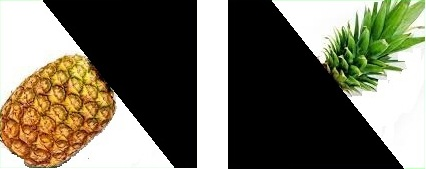
\includegraphics[scale=0.5]{images/region1and2}
		\captionof{figure}{Left: First Region or \(x' > cp\), Right: Second Region or  \(x' <= cp\)}
	\end{center}
	\begin{center}
		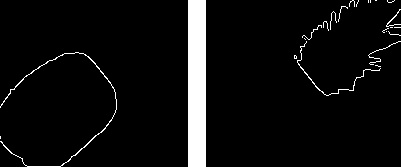
\includegraphics[scale=0.5]{images/image_gradient}
		\captionof{figure}{Image Gradient (Canny Algorithm)}
	\end{center}
\end{multicols}

Compactness calculation involves the perimeter. The perimeter was obtained through edge detection operations. In this study, edge detection was done using a canny algorithm. Szeliski (2011) \cite{Szeliski:2011} defines the edge as an area that gradually changes the intensity of pixels. Especially for the canny algorithm, it usually applies gradient analysis, followed by hysteresis and non-maximum suppression. However, this study did not implement them because the processed image was a binary image. Without both processes, the resulting edge of the object is clear. After the perimeter for each region was obtained, the compactness was calculated for the first (\(c1\)) and the second (\(c2\)) region based on \(\textbf{Equation 2}\). The determination of an area as fruit or crown was done based on the following figure.

\begin{center}
	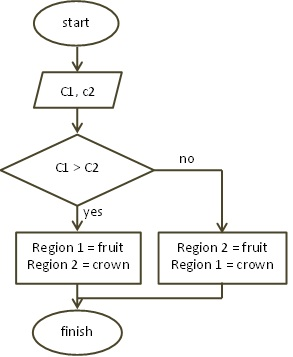
\includegraphics[scale=0.73]{images/fruit-recognition-flowchart}
	\captionof{figure}{Fruit and Crown Recognition Flowchart}
\end{center}

\subsection{Ripeness Index Classification}
In the previous section, this paper already described the methods of the pineapple crown and fruit separation subtopic. In this section, we will focus on the next subtopic that is ripeness classification. 
	
\subsubsection{Ripeness Standard}
The ripeness standard in this study is referring to the industry standard released by Sunpride. Sunpride is the third largest pineapple producer in the world located in Lampung Province, Indonesia. The pineapple ripeness index, according to Sunpride, consists of four levels, namely 1, 2, 3, and 4. In this paper, also referred to as classes A, B, C, and D.

\subsubsection{Fruit Color Extraction}
After the computer can recognize the fruit and crown region, The fruit color extraction was done. \textbf {Figure 9} shows the process of fruit color extractions.
\begin{center}
	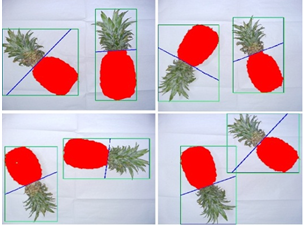
\includegraphics[scale=0.73]{images/color-extraction}
	\captionof{figure}{Extracted Fruit Pixels (Red Color))}
\end{center}
Each extracted pixel is given a red color as a marker. The R, G, and B of the fruit are the mean values of the object pixels. Then these values were derived into other components, namely I, H and S. I is the intensity of the color obtained by the following equation,
\begin{equation}
	I = \frac{R + G + B}{3}
\end{equation}
Intensity describes the lux of lighting or brightness of the image. By including this factor, we expected that the resulting model has better flexibility to the change of the lighting levels. Besides intensity, we also get saturation. This parameter describes the level of concentration and  obtained from the following equation,
\begin{equation}
	S = 1- \frac{1}{I}
\end{equation}

\subsubsection{Classification Algorithm}
The ripeness level is classified using a backpropagation neural network (BPNN). Inputs of this neural network are fruit colors which consist of RG, RGB, RGBI, RGI, HSI, and RGBHSI. The neural network architecture used in this study shown in Figure 10. The architecture consists of a layer of input neurons, hidden layers, and an output layer. The hidden layer uses the rectified linear unit (Relu) as an activation function, and the output layer uses the softmax. The learning rate was 0.0001. During the training process, the stored model is the model with the best test accuracy before overfit. In this study, there are 552 datasets. The result reported in this research is the test accuracy. 
\begin{center}
	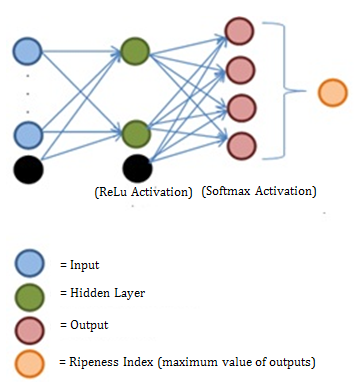
\includegraphics[scale=0.6]{images/net}
	\captionof{figure}{Neural Network Architecture)}
\end{center}

\section{Result and Discussion}
In this part, this paper will discuss the performances of the pineapple crown and fruit recognition, the ripeness classification, and the final result.
 
\subsection{Pineapple Crown and Fruit Recognition}
In this section, this paper will focus on discussing the performance of pineapple fruit and crown separation. As presented before, this research is utilizing a compactness feature for that objective. Compactness describes the regularity of the surface of an object. In relation to the pineapple, the fruit surface is more regular than the crown. So the value of the fruit compactness is higher than the crown. The figure below shows the differences between the compactness of the fruit and the crown from 100 object samples.
\begin{center}
	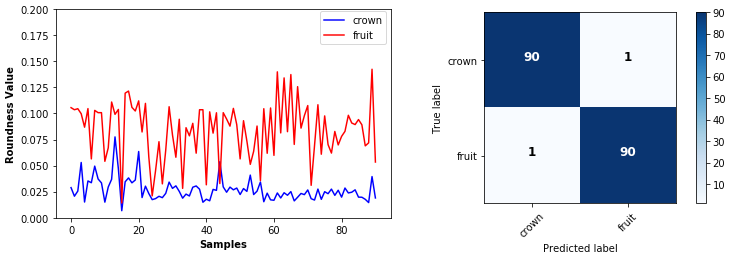
\includegraphics[scale=0.8]{images/sparation-result}
	\captionof{figure}{Left: Compactness Values   Right: Confution Matrix of Pineapple Fruit Recognition)}
\end{center}

Based on the graph above, it is evident that the compactness value of the fruit is always higher than the crown. However, there is an outlier due to the defect of the crown shape or the imperfect binary process. With this method, the computer can recognize the fruit and the crown with 98.92\text{\%} of accuracy as shown in \textbf{Figure 11} on the right side. Besides, the recall value for each class is 98.92\text{\%} too. These results indicate this method is acceptable for separating the fruit and crown region of pineapple. This ability is crucial and fundamental for further process, such us ripeness classification. Ripeness classification requires feature extractions in the part of the fruit, so it is very dependent on the fruit separation result. Without this capability, the extraction of fruit color is impossible. Some previous researches overcome this by cutting the crown first and causes the pineapple to rot quickly.

\subsection{Ripeness Index Classification: Feature Engineering}
After the computer can identify the part of the fruit and crown, color features were extracted from the fruit for ripeness classification. The ripeness standard of this study is the Sunpride standard. The figure below shows the distribution of the extracted colors of this study.
\begin{center}
	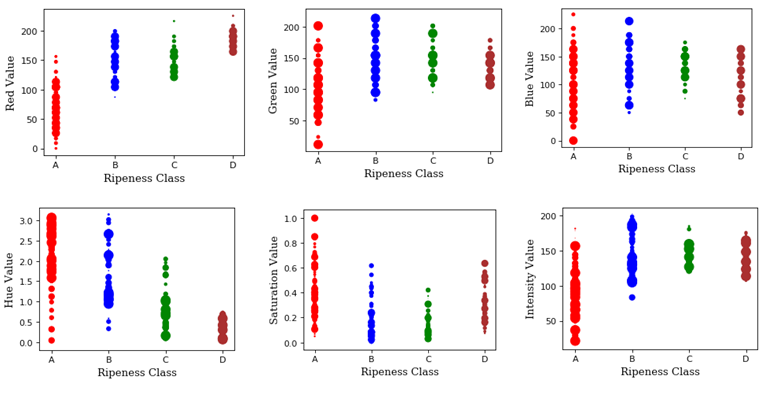
\includegraphics[scale=0.65]{images/colors}
	\captionof{figure}{ Color Values for Each Class)}
\end{center}
From the picture above, this study gets a piece of information that there is no single parameter able to classify each class. Consequently, the manual threshold method cannot be used for this classification. To overcome this problem, we used the neural network as a classifier.
Furthermore, we have to select the proper features for neural network inputs. In this study, we analyze the correlations between the color components and the target classes. The results show that the red feature has the best correlation (0.8122) to the ripeness level. Then the intensity component in the second place (0.57), followed by green and hue. After that, we have to ensure that these inputs are good enough for the classification. So, this research utilized a T-SNE method to investigate it. T-SNE describes the distribution of input features for each class by reducing the dimension into two main components. The figure below shows the result of this study.
\begin{center}
	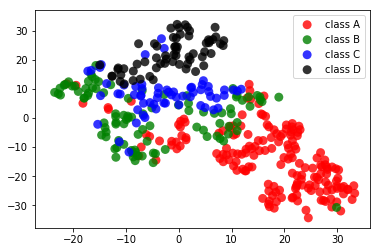
\includegraphics[scale=0.55]{images/tsne}
	\captionof{figure}{Feature Distribution from T-SNE Algorithm}
\end{center}
Based on the picture above, this research gets a piece of information that the extracted features are sufficient for pineapple ripeness classification. This figure proves that the combination of input features for each class are separated clearly.

Based on the expert point of view, intensity describes the level of illumination. It is becoming a piece of complementary information on red and green features. By entering this feature, we expected to get a robust model against the light changes. This information is useful for neural network input design. For this research, the combinations of the tested input features are RG, RGB, RGBI, RGI, HSI, and RGBHSI.

\subsection{Ripeness Index Classification: Training}
This study compared the accuracy chart to get the best input combination, as shown by the figure below. The graph illustrates the changes in accuracy for each iteration. It also describes the maximum accuracy achieved by each input combination. The best input is the combination with the highest accuracy with a fast increment for each iteration. The chart presented below is the test accuracy chart. The main reason for using the test accuracy is the capability to describe the real performance of the algorithm. It happens because the test accuracy is free from overfitting. Overfitting is a condition where the actual ability of the algorithm continues to decrease, but the accuracy of the training continues to rise, even near perfect. This paper also presents the training chart as a comparison.

\begin{center}
	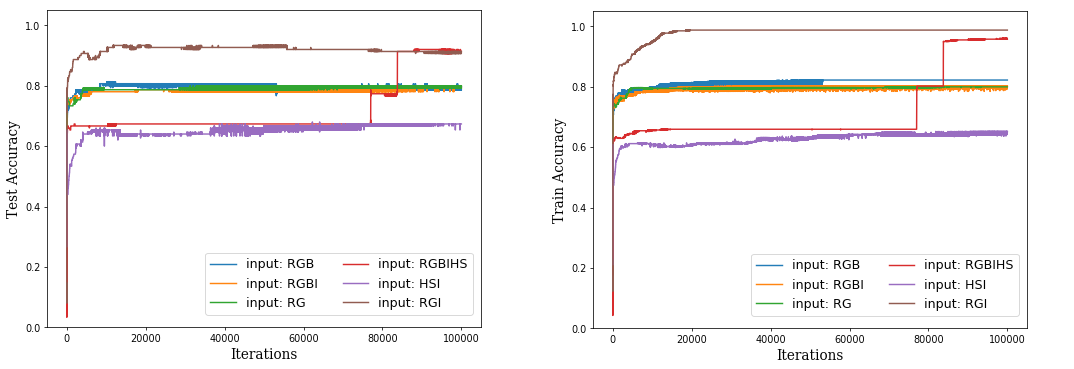
\includegraphics[scale=0.65]{images/test-result}
	\captionof{figure}{ Test and Train Accuracy}
\end{center}

Based on the graph above, this study gets information that the RGI input has the best classification capability, with 93.33\text{\%} of test accuracy. Followed by RGBHSI input with a test accuracy of 92\text{\%} in the second position. While the RG, RGB, and RGBI inputs are in the range of 80\text{\%}, and HSI only reaches 63\text{\%}. Besides, RGI inputs also the best in the aspect of their accuracy increment in each iteration. From the test graph, this input reaches the value above 90\text{\%} less than 2000 epochs, then starts to overfit. It is marked by the value of the accuracy of the test decreases slowly, while the accuracy of the training is stagnant at 96\text{\%}. This achievement is very different from RGBIHS input. RGBIHS requires 8000 more epochs to achieve the test accuracy of 90\text{\%}. The model stored in this study is the highest accuracy occurring before overfitting.


\begin{center}
	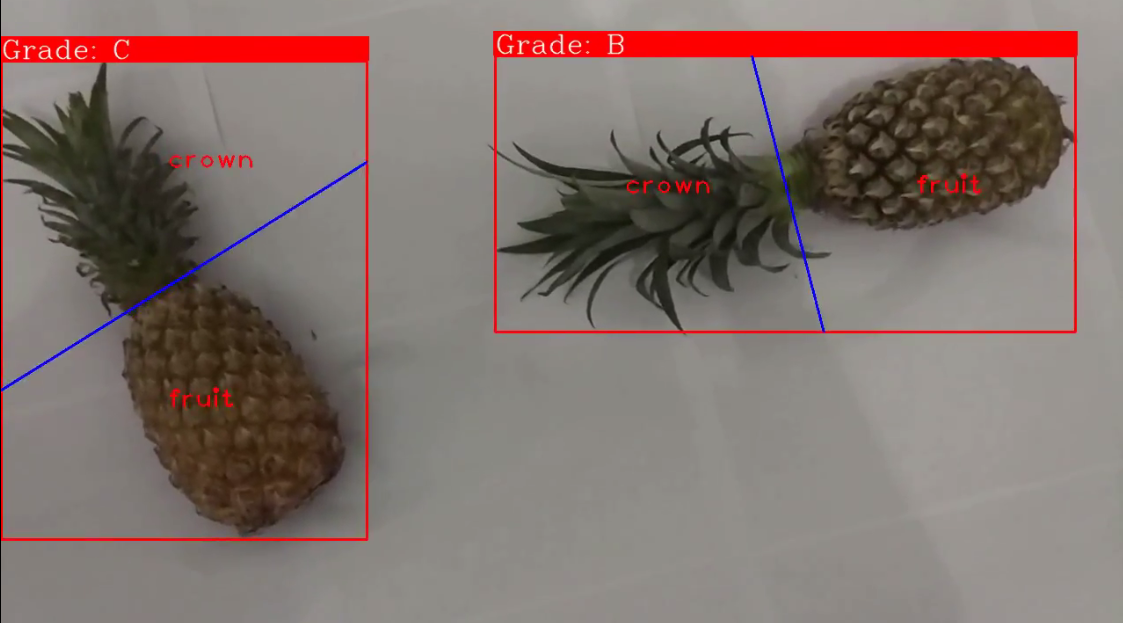
\includegraphics[scale=0.3]{images/final-result1}
\end{center}

\begin{center}
	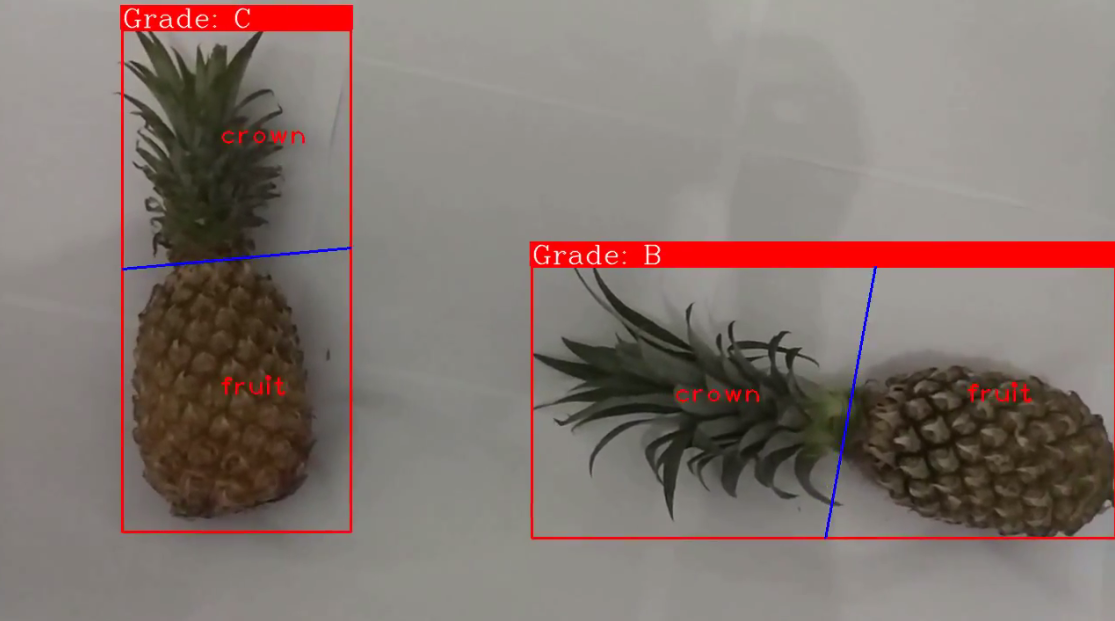
\includegraphics[scale=0.3]{images/final-result2}
	\captionof{figure}{Final Result with RGI as an Input}
\end{center}

\subsection{Computation Time}
In this section, this paper will present the end to end computation time performance of the algorithm. The FPS (frame per second) is analyzed by averaging the process in all frames in a video. The results of this performance are presented by the table below.

\begin{tabular}{ p{1.7cm} p{1.7cm} p{3.3cm} p{1.8cm} p{1.8cm}}
	\hline
	Experiment & Number of Obejct per Image & Object Size (Pixels) & Processing Time (ms) & FPS\\
	\hline
	1.& 1 & $616797\pm38808$ & $48.4\pm6.5$ & $20.7\pm2.8$\\ 
	2.& 1 & $281940\pm12777$ & $36.8\pm6.7$ & $27.2\pm5.0$\\
	3.& 1 & $230486\pm3699$  & $35.9\pm6.4$ & $27.8\pm5.0$\\
	4.& 2 & $199144\pm30806$ & $37.5\pm3.7$ & $26.7\pm2.6$\\
	5.& 2 & $106663\pm7164$  & $37.9\pm9.0$ & $26.3\pm6.2$\\
	\hline
\end{tabular}

Our algorithm reaches 27 FPS in the end to end performance, and fast enough for real-time application, such as in a belt conveyor grading system. This achievement is far better than the 3 FPS achieved by Kaewapichai et. al. The other previous methods didn't report the end to end performance because of their researches only focus on a still image application, or just laboratory scale. With this achievement, our method is capable of real-time use in industry and become the second breakthrough offered from this research.

\section{Conclusion}
This study provides a new technique for vision-based pineapple quality classification. This technique makes a computer able to separate the part of the crown and fruit automatically. So, it allows a vision-based pineapple quality evaluation without having to cut the crown first like previous studies. This method is suitable for indoors with a homogeneous background classification. The capability is 180/182 of accuracy with 90/91 of recall for the fruit and crown recognition. These results are acceptable as a fundamental step for the next process. For the ripeness classification, the highest accuracy is RGI input with a test accuracy of 93.33 \text {\%}. It happens because the color of red (R) and green (G) are more correlated to the level of ripeness than others. Besides, the intensity (I) completes the value of R and G because describes the intensity of lighting.

\bibliography{btxdoc}
\bibliographystyle{plain}
\end{linenumbers}
\end{document}
